%%%%%%%%%%%%%%%%%%%%%%%%%%%%%%%%%%%%%%%%%%%%%%%%%%%%%%%%%%%%%%%%%%
%%%%%%%% ICML 2015 EXAMPLE LATEX SUBMISSION FILE %%%%%%%%%%%%%%%%%
%%%%%%%%%%%%%%%%%%%%%%%%%%%%%%%%%%%%%%%%%%%%%%%%%%%%%%%%%%%%%%%%%%

% Use the following line _only_ if you're still using LaTeX 2.09.
%\documentstyle[icml2015,epsf,natbib]{article}
% If you rely on Latex2e packages, like most moden people use this:
\documentclass{article}

% ams packages
\usepackage{amsmath,amsfonts,amssymb}

% use Appendix
\usepackage{appendix}

\usepackage{multicol}

% use Times
\usepackage{times}
% For figures
\usepackage{graphicx} % more modern
%\usepackage{epsfig} % less modern
\usepackage{subfigure} 

% For citations
\usepackage{natbib}

% For algorithms
\usepackage{algorithm}
\usepackage{algorithmic}

% As of 2011, we use the hyperref package to produce hyperlinks in the
% resulting PDF.  If this breaks your system, please commend out the
% following usepackage line and replace \usepackage{icml2015} with
% \usepackage[nohyperref]{icml2015} above.
\usepackage{hyperref}

% Packages hyperref and algorithmic misbehave sometimes.  We can fix
% this with the following command.
\newcommand{\theHalgorithm}{\arabic{algorithm}}

% Employ the following version of the ``usepackage'' statement for
% submitting the draft version of the paper for review.  This will set
% the note in the first column to ``Under review.  Do not distribute.''
%\usepackage{icml2015} 

% Employ this version of the ``usepackage'' statement after the paper has
% been accepted, when creating the final version.  This will set the
% note in the first column to ``Proceedings of the...''
\usepackage[accepted]{icml2015}


% The \icmltitle you define below is probably too long as a header.
% Therefore, a short form for the running title is supplied here:
\icmltitlerunning{10-708 PGM Project Final Report: Learning SNP-Gene Network Using Mixed Graphical Model}

\begin{document} 

\twocolumn[
\icmltitle{10-708 PGM Project Final Report \\ 
           Learning SNP-Gene Network Using Mixed Graphical Model}

% It is OKAY to include author information, even for blind
% submissions: the style file will automatically remove it for you
% unless you've provided the [accepted] option to the icml2015
% package.
\icmlauthor{Hyun Ah Song}{hyunahs@andrew.cmu.edu}
\icmladdress{Machine Learning Department, Carnegie Mellon University, Pittsburgh, PA 15213}
\icmlauthor{Ji Oh Yoo}{jiohy@andrew.cmu.edu}
\icmladdress{Computer Science Department, Carnegie Mellon University, Pittsburgh, PA 15213}

% You may provide any keywords that you 
% find helpful for describing your paper; these are used to populate 
% the "keywords" metadata in the PDF but will not be shown in the document
\icmlkeywords{boring formatting information, machine learning, ICML}

\vskip 0.3in
]

\begin{abstract} 
Learning eQTL mapping between SNPs and expression rates of related proteins is important in discovering the key factors of diseases. Most previous attempts require the prior knowledge in gene expression rates or include unnatural assumptions in the encoding of SNPs. In this project, we propose conditional mixed graphical model for SNPs-gene network learning to resolve these limitations. Our approach models SNPs as discrete values to relax the unnatural assumption and does not require the prior knowledge. Our model outperforms previously proposed methods in synthetic experiment settings. Results on Human Liver Cohort dataset show that our model does not perform better than the previous methods due to the relatively high sample complexity, and it requires further analysis on the behavior of our model.
\end{abstract} 

\section{Introduction}
Recent progress on large scale genome-wide studies show that many human common diseases, including diabetes, asthma, and cancer, consist of complex reactions of proteins, which are controlled by regulatory networks and are expressed from highly correlated genetic variations \cite{basso2005reverse, chen2008variations}. Thus, rather than simple correlation studies between a few clinical phenotypes and genetic variations of interest, discovering eQTL mapping between the multiple genetic variations and multiple disease-related proteins' expression rates is necessary to analyze the occurrence mechanism of the diseases and the functional roles of those proteins in the mechanism. This requires the joint learning of the genetic variations and the expression of the related proteins rather than combining the results from the independent study on each genome or phenome. Multiple regression studies have been conducted to identify these mappings between single-nucleotide polymorphisms (SNPs) and related gene expression rates, and to develop the more efficient and accurate methods for this eQTL mappings discovery \cite{kim2010tree, sohn2012joint}. We adopt conditional undirected mixed graphical model \cite{lee2013structure} for SNP-gene network learning to relax the assumptions and lessen requirements for learning in the previous methods, and analyzed the performance of our model in both synthetic environment and real-world application.




\section{Background \& Related Work}
\label{LiteratureReview}


\subsection{Related Work}
There have been various types of solutions to the problem of learning SNPs-gene network. One popular solution is to solve the problem as multiple-output regression, a straight-forward extension of single-output regression. 
Given SNPs information as inputs, multiple-output regression tries to solve the regression task for each output simultaneously while sharing the coefficient matrix for all the tasks. It can incorporate L-1 penalty (lasso) for sparse model and L-21 mixed penalty for desired sparsity pattern in the coefficient matrix \cite{obozinski2008high}.




Tree-guided group lasso, or GFlasso was proposed by Kim and coworkers \cite{kim2010tree}.
GFlasso aims to learn the common set of inputs for each cluster of outputs, using group lasso penalty and systematic weighting scheme for inputs, where inputs are grouped together to be mapped to the outputs, and output clusters with strong correlation are guided to share common input groups.
GFlasso requires the prior knowledge of output tree structure, which is not always possible.
Also, the weighting scheme of guiding the common set of inputs for highly correlated clusters is such a strong assumption that may not be true in reality.


An algorithm called multivariate regression with covariance estimation (MRCE) that aims to learn both multivariate regression parameters and the correlation of outputs was introduced by Rothman and coworkers \cite{rothman2010sparse}.
By regularizing regression parameter and correlation matrix separately, the MRCE solve bi-convex problem, which may not lead to the global optimum. Although MRCE is favorable in a way that it learns the output structure, MRCE does not force structured sparsity when learning regression parameters for inputs, which is an important property when dealing with SNPs-gene data.


An algorithm that bring together the advantages of the two previous works \cite{kim2010tree} \cite{rothman2010sparse} was introduced by Sohn and coworkers \cite{sohn2012joint}. 
The proposed algorithm jointly learns regression parameters and output structure with constraint of structure sparsity in inputs, by learning conditional Gaussian graph model.
Although proposed algorithm resolves the main problems in previous studies, it assumes that input and output are treated as continuous data, which is not true for SNPs-gene data.
Therefore, it leaves some space for further refinement of the assumptions used in this algorithm.









In order to solve the problem in more natural way, we can adopt 'mixed graphical models' into our problem.
Mixed graphical models refer to graphical models that allow for both discrete and continuous variables.


Lauritzen first proposed a mixed graphical model for variables of both discrete and continuous \cite{lauritzen1989graphical}.
 Although this mixed graphical model is carefully designed for general cases, this makes resulting conditional distribution complex. Also, the mean and covariance matrices exist for every possible configurations of states of discrete variables, which results in exponential increase in number of parameters to learn depending on the number of discrete variables.




Later by Jason and coworkers, the mixed graphical model was further developed into more simplified and intuitive version \cite{lee2013structure}. 
The authors proposed a mixed graphical model that provides intuitive forms of conditional distributions: conditional distribution of a discrete variable reduces to multi-class logistic regression, and that of a continuous variable to Gaussian linear regression. 
By making assumptions on the general mixed graphical models  \cite{lauritzen1989graphical}, proposed algorithm scales up more efficiently: it has common covariance matrix, and additive mean.


To our knowledge, there has not been any study that learns the SNP-gene network as multi-task regression problem using mixed graphical models. 
In this project, we would like to extend the basic concepts proposed by Sohn  \cite{sohn2012joint} using mixed graph models \cite{lee2013structure}, to solve the problem in more natural way.







\subsection{Background}
One of the most commonly used method in estimation of SNP-gene network is the multiple-output extension of single-output regression method with lasso penalty \cite{tibshirani1996regression}, which solves the following optimization problem.

\begin{align}\label{eq:lasso}
\text{arg} \min_{\textbf{B}} \text{tr}((\mathbf{Y}-\mathbf{XB})(\mathbf{Y}-\mathbf{XB})^T) + \lambda \| \mathbf{B}\|_1,
\end{align}

where $\mathbf{X}=(\mathbf{x_1}, ... ,\mathbf{x_N})^T$, $\mathbf{Y}=(\mathbf{y_1}, ... ,\mathbf{y_N})^T$ are input and output data, and $\mathbf{x_i}=(x_{i1}, ... ,x_{iJ})^T \in \mathbb{R}^J$, and $\mathbf{y_i}=(y_{i1}, ... ,y_{iK})^T \in \mathbb{R}^K$.
The output is estimated by regression: $\mathbf{y_i}=\mathbf{Bx_i}+\mathbf{\varepsilon_i}$, where $\varepsilon  \sim \mathcal{N}(0, \mathbf{\Psi})$.
By enforcing sparsity in \textbf{B}, it is able to take into account of the problem setting that we have $J >> N$, where the number of SNPs is higher than the number of samples. Also, using L-1/L-2 mixed norm penalty can be used for joint feature selection \cite{obozinski2008high}.


Despite the simple formulation and optimization method for multiple-output regression, it does not capture the relatedness among the output variables in the data. To address this problem of learning structured sparsity and structure in output variables, Graph-guided Fused Lasso is developed with fusion penalty according to pre-computed degree of relatedness among the output \cite{kim2009statistical}, but it needs prior knowledge of the data, which can differ by each problem setting and its problem domain. To overcome this problem of necessity of prior knowledge, Sohn and coworkers proposed Sparse Conditional Gaussian Graphical Model, which extends the problem of learning standard regression model into learning a conditional Gaussian graphical model \cite{sohn2012joint}. It assumes that the joint distribution of input and output as a single multivariate Gaussian distribution as Eq. \ref{eq:jointG}.

\begin{align}\label{eq:jointG}
\begin{split}
\begin{bmatrix}
    \mathbf{x_i}\\
    \mathbf{y_i}
\end{bmatrix}
 \sim \mathcal{N}
 \begin{pmatrix}
\begin{bmatrix}
    \mathbf{0}_J  \\
   \mathbf{0}_K
\end{bmatrix}
,
    \Sigma
\end{pmatrix} \\
\mathbf{\Sigma}^{-1}= \begin{pmatrix}
    \mathbf{\Theta}_{xx} & \mathbf{\Theta}_{xy}\\
   \mathbf{\Theta}_{xy}^T &  \mathbf{\Theta}_{yy}  
\end{pmatrix}
\end{split}
\end{align}
Then, the parameters $\Theta$ and $\Phi$ in Eq. \ref{eq:lasso} can be reconstructed by $\mathbf{B}=\mathbf{\Sigma}_{xy}^T \mathbf{\Sigma}_{xx}^{-1}=-\mathbf{\Theta}_{yy}^{-1}\mathbf{\Theta}_{xy}^T$, and $\mathbf{\Psi}= \mathbf{\Theta}_{yy}^{-1}$.

Although this method by Sohn suits the needs for the SNP-gene network estimation problem as it learns both structured sparsity in $\Theta$ and output structure in $\Phi$, and formulates the problem using the standard regression problem, the underlying assumption is that both input and output data constitute of continuous variables. This assumption is from that the degree of genetic variation, the deviation from major alleles, can be measured by the number of minor alleles in a person's genotype, and the relationship between the deviation and output is linear. However, the phenotypes from genes with 0 or 1 minor alleles can be drastically different from those of 2 minor alleles in many cases including examples from Mendel's Law.  Thus, it is reasonable approach to relax this assumption in the previously developed regression models and model the SNPs as categorical, discrete values.

As with the previous models, continuous variables can be modeled as a multivariate Gaussian: $y \sim \mathcal{N}(0, \Theta^{-1})$, where the inverse covariance matrix $\Theta$ can be estimated via graphical lasso. For discrete variables, pairwise Markov random field $p(x) \propto exp \sum_{r\leq j} \phi_{rj}(x_r, x_j)$ is one of the commonly used graphical model.
Studies on mixed graphical model, which combines two commonly used graphical models of Gaussian and pair-wise graphical models so that it can handle data consisting of both continuous and discrete variables, have been conducted by Lauritzen and coworkers, where the conditional distribution is modeled as $p(y|x) = \mathcal{N}(\mu(x), \Sigma(x))$ \cite{lauritzen1989graphical}.
Despite of the novelty and specific applications of the mixed graphical model, it has not been used as widely due to its complexity in learning the parameters, and lack of intuition when derived to the other types of distributions.

Lee and coworkers \cite{lee2013structure} have proposed a special case of the mixed graphical model that resolves the problem of the complexity in parameter learning and vague forms of derived distributions by making several assumptions.
 The detailed explanation follows in section \ref{Methods}.
 
In our work, we investigate the performance of conditional mixed graphical model, whose assumption on the types of data it can handle does not violate our problem setting for SNP-gene network estimation. We compare the performance of the mixed graphical model when applied to SNP-gene network estimation problem, and that of commonly used method.


\section{Methods}
\label{Methods}
Our goal is to improve the method of learning SNP-gene network by adopting the conditional undirected mixed graphical model in which we can embed both discrete variables for SNPs and continuous variables for gene expression rates.

\subsection{Mixed Graphical Model}
Lee and coworkers \cite{lee2013structure} proposed a mixed graphical model of discrete and continuous variables, where the joint distribution is expressed as:

\begin{align}
p(x, y ; \Theta) \propto \exp \Big( &\sum_{k=1}^{q} \sum_{l=1}^{q} \phi_{kl} (x_k, x_l) \nonumber \\
+ \sum_{k=1}^{p} \sum_{s=1}^{q} \rho_{ks}(x_k) y_s  &+ \sum_{s=1}^{p} \alpha_s y_s + \sum_{s=1}^{p} \sum_{t=1}^{q} -\frac{1}{2} \beta_{st} y_s y_t \Big) \label{eq:joint}
\end{align} 

where $x_1, ... x_p$ are discrete variables representing the occurrences for each SNP and $y_1, ..., y_q$ are continuous variables representing the gene expression rate of each gene. 
The parameters are $\Theta = [\{\phi_{kl}\}, \{\rho_{k}\}, \{\alpha_{s}\}, \{\beta_{st}\}]$, where $\phi_{kl}$, $\rho_{k}$, $\alpha_{s}$, $\beta_{st}$ are the discrete-discrete edge potential, continuous-discrete edge potential, continuous node potential, and continuous-continuous edge potential, respectively.

By making further assumptions on mixed graphical models originally introduced in \cite{lauritzen1989graphical}, the mixed graphical model \ref{eq:joint} proposed by Lee \cite{lee2013structure} yields intuitive results when reformulated into various forms of distributions. The conditional distribution of continuous variables and discrete variables given the rest reduces to Gaussian linear regression, and multi-class logistic regression, respectively. Furthermore, when the data consists of continuous and discrete variables only, the model reduces to multivariate Gaussian model, and pairwise discrete Markov random field, respectively. 

\subsection{Conditional Mixed Graphical Model}
We are interested in learning the SNP-gene network structure, and the conditional distribution of the gene expression, given observed SNPs.
Therefore, we only need to focus on learning the conditional distribution of the network rather than learning the full joint distribution. 

The conditional distribution of continuous variables given discrete variables of the mixed graphical model in \cite{lee2013structure} reduces to the form of multivariate Gaussian distribution.

\begin{align}
p(y|x) &= \mathcal{N}(B^{-1}\gamma(x), B^{-1}) \label{eq:cond_prob}\\
\{\gamma(x)\}_s &= \alpha_s + \sum_{k} \rho_{ks}(x_k) \\
p(x) &\propto \exp \Big( \sum_{k} \sum_{l} \phi_{kl}(x_k, x_l) + \frac{1}{2} \gamma(x))^\intercal B^{-1} \gamma(x) \Big)
\end{align}

where $B$ is a symmetric, positive definite inverse covariance matrix $B = \{ \beta_{st}\}$ that is shared across the Gaussian distributions. 

From the property of multivariate Gaussian distribution, the log likelihood of the parameters $\Theta$ given discrete variables $y$ can be expressed as:
\begin{align}
\log p(y | x; \Theta) &= -\frac{1}{2}\log |B^{-1}| -\frac{k}{2} (2 \pi) \nonumber    \\
& -\frac{1}{2} (y - B^{-1} \gamma(x)^\intercal B (y - B^{-1} \gamma(x)) \label{eq:loglikli} \\ 
l_p(\Theta) &= -\frac{1}{2} tr\Big((Y - B^{-1} \Gamma(X))^\intercal B (Y - B^{-1} \Gamma(X)) \Big) \nonumber \\
& -\frac{N}{2} \log|B^{-1}| + \lambda_1 \|\{\beta_{st}\}\|_1 + \lambda_2 \|\{\rho_{ks}\}\|_1 \label{eq:obj}
\end{align}

The parameter $\Theta^*$ that minimizes this L-1 penalized log-likelihood will give us a sparse and consistent estimator, and by comparing the parameters with results in multi-task regression settings, we can analyze the existence of direct and indirect relationship between SNPs and gene expression rates.

For the parameter estimation, we minimize the negative log-likelihood expressed in product of each variable given the rest as follows:
\begin{align}
\tilde{l}(\Theta |y) = - \sum_{s=1}^{p} \log p(y_s |y_{\setminus s}, x;\Theta),
\end{align}
where from \ref{eq:joint}, $p(y_s |y_{\setminus s}, x;\Theta)$ can be reformulated as follows:
\begin{align}
&p(y_s |y_{\setminus s}, x;\Theta) =\nonumber    \\
& \frac{\sqrt{\beta_{ss}}}{\sqrt{2\pi}} \exp \left(\frac{-\beta_{ss}}{2} \left(y_s - \frac{\alpha_s + \sum_j \rho_{sj}(y_j)-\sum_{t=s}\beta_{st}y_t }{\beta_{ss}}\right) \right)^2
\end{align}




\subsection{Optimization}
For the optimization, proximal Newton method \cite{schmidt2010graphical,schmidt2011projected} is used. Proximal Netwon optimization method breaks down the optimization problem into $f(x) + g(x)$, where $f(x)$ is smooth and convex function, and $g(x)$ is a convex function, but not necessarily smooth. 
In our problem, functions $f(x)$ and $g(x)$ correspond to the negative log-likelihood and sparsity constraint, respectively.

Proximal Newton method is an extension of proximal gradient method that considers the second order information of $f(x)$ instead of the first order.
The proximal gradient seeks next point by computing $x_{k+1} = prox_t (x_k - t \bigtriangledown(x_k))$, where $prox_t(x)=\text{argmin}_u(\frac{1}{2t}{\|x-u\|}^2 + g(u))$, and $t$ is chosen by Armijo line search algorithm. In proximal Newton method, $Hprox$ is used, where the $prox$ operator is extended to $\| \cdot \|_H$, where $H=\bigtriangledown^2 f(x_k)$. For each iteration, proximal Newton method finds the next point that minimizes below function.
\begin{align}
  &\bigtriangledown f(x_k)^T(u-x_k)+\frac{1}{2t}(u+x_k)^TH(u-w_k)+g(u) \nonumber    \\
 & =  Hprox_t(x_k-tH^{-1}\bigtriangledown f(x_k)).
\end{align}

Previous studies on proximal Newton method \cite{lee2012proximal} shows that it converges faster especially when $n$ is large, with better accuracy compared to the proximal gradient method.

For the implementation, $H$ is approximated using BFGS.
We used PNOPT package \cite{lee2012proximal} for implementation of proximal Newton optimization algorithm.



\section{Experiments}


% % % begin
% % % added for final
\subsection{Synthetic Experiments}
Before delving into real-world dataset, we run experiments on synthetic data to verify our assumptions on the behavior of our proposed model.


\subsubsection{Synthetic Data Generation}
We create a simple model as a ground truth with 7 discrete variables (input) and 5 continuous variables (output).
We design the discrete variables to have three possible states to reflect the nature of SNP-gene data. We construct a chain structure for the discrete variables, where each node is linked to the following node. For two consecutive nodes that are connected by an edge, we randomly make a state-to-state interactions as following.

\begin{align*}
\centering
0.5 * 
\begin{bmatrix}
  1 & 0 & -1 \\
  0 & 1 & 0 \\
  -1 & 0 & 1
\end{bmatrix}
\end{align*}

The continuous variables are designed to have symmetric interactions between the nodes, where we generate random values for node-to-node interaction in range of [-1 1], and remove the edge with probability of $0.7$ until the matrix becomes positive semi-definite.

For the input-output interaction, we randomly create edges with probability of $0.2$. 
In order to reflect our assumption on the nature of SNP-gene data, and therefore verify that our proposed model excels in performance under this assumption, we design the interactions between the discrete and continuous variables that are linked via an edge to be increasing in non-linear manner with respect to the index of the states;
we define the interactions between three states of the discrete variable and the continuous variable to be in non-linear relationship as follows: [1 1.2 6].



 Total 2000 samples are sampled from the true model and used for estimating the edges between the discrete variables and the continuous variables. 
 We analyze the performance based on the two measures: prediction error (mean squared error of predicted output) in section and accuracy of edge discovery (true positive and true negative out of total number of edges). 
We repeat the experiment for 10 times by randomly splitting 2000 samples into training set ($80 \%$) and test set ($20\%$), and average the prediction error.
 To find the optimal hyper-parameters, we use 3-fold cross-validation based on the prediction errors.
 
 
 
 
 

\subsubsection{Prediction Error}

The prediction errors of proposed method, sparse CGGM, lasso, and multi-task lasso are shown in Table \ref{table:syn_pred_err}.
Our proposed method achieves the lowest prediction error, followed by multi-task Lasso, Lasso, and SCGGM, where SCGGM achieved worst prediction with largest variation.
We can clearly see that multi-task lasso and lasso perform better prediction than SCGGM.
The lasso family is expected to learn non-linear input-output relationships by making approximations to linear weights across the states via interpolations.
Compared to lasso family, learning of SCGGM model takes more intricate procedures, which may have resulted in more confusion in incorporating non-linearity into the parameter learning.
From this experimental result, we can conclude that under given assumptions on the data, where non-linear relationships between the states of input and output variables are expected, our proposed model takes advantage of the model structure, and conducts parameter learning in more desired manner.



 
\begin{table}[hbtp]
\begin{center}
    \begin{tabular}{| c | c |}
    \hline
    Method & Prediction Error \\
    \hline
    \textbf{MG} & $\mathbf{1.4798 \pm 0.1811}$ \\
    SCGGM & $2.1308 \pm 0.5252$  \\
    Lasso & $1.8394 \pm 0.2107$  \\
    MTLasso & $1.7950 \pm 0.1625$ \\
    \hline 
    \end{tabular}
\end{center}
 	\caption{Prediction error on synthetic dataset with methods MG (mixed graphical model), SCGGM (sparse CGGM), Lasso, MTLasso (multi-task Lasso).}
 \label{table:syn_pred_err}
\end{table}



\subsubsection{Edge Recovery}
Making better predictions on gene expression based on the SNPs data is an important task in learning SNP-gene network. However, learning of the data structure itself that reveals the relationships between the SNPs-gene expression or gene expressions themselves is of great interest as making better predictions. Considering the task of structure learning, graph-based models are considered more powerful and meaningful, compared to lasso-based models.

Using the same setting for the data generation, we assess how well our model and SCGGM, another graph-based model, learns the true data structure.
We analyze the dependency of the structure learning on the sample size, by computing the accuracy of the edge recovery rate of the input-output network with varying number of samples used for model learning.
We increase the number of sample size by 250 interval until 2000.
The experimental results are averaged over five repeated trials.
(Both our proposed method and SCGGM do not learn sparse-enough parameters for input-output network structure, so we threshold the recovered parameters over certain values (1 for proposed method, and 0.001 for SCGGM) to finally attain meaningful network structures.)

Figure \ref{fig:syn_edge_rec} shows the edge recovery rate of our proposed method (Mixed Graphical model - MG), and SCGGM.
We see that for the sample size of 250, SCGGM achieves slightly better edge recovery. 
As we increase the number of sample size, our proposed method shows improvement in edge recovery rate, and converges to 1 with 750 samples. 
On the other hand, SCGGM does not show any improvement over incremental sample size.
The interpretation of the result is straightforward.
Since our proposed method is capable of managing the non-linearity in the data structure, it shows expected learning curve based on the sample size.
For SCGGM, since the structure learning is not being done as desired, increasing the sample size does not resolve the intrinsic problem of ill-learning of the model structure.

\begin{figure}[h]
  \centering
  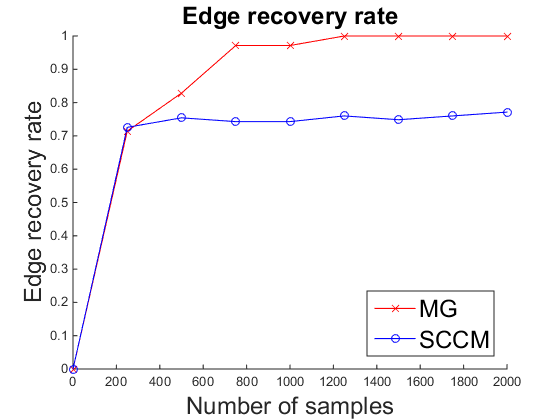
\includegraphics[width=3in]{figure/EdgeRecRate2.png}
  \caption[] {Edge recovery rate of MG and SCGGM on the synthetic dataset.\label{fig:syn_edge_rec}}
\end{figure}


In Figure \ref{fig:interactions}, images of input-output, and output-output structures learned by proposed method and SCGGM are displayed with ground-truth.
Each row shows the images of ground-truth, outcomes of proposed method, and SCGGM when the sample size is 2000, respectively.
First two columns are outcomes of input-output network structures, and the third column is for output-output network structure. 
Each of the first two columns shows raw parameters, and binarized parameters over threshold.

We see that even when sufficient number of samples are provided for model learning, while proposed method learns and recovers perfect ground-truth input-output network structure, SCGGM fails to recover the true network structure. 
For the network structure of output-output relationships, both proposed method and SCGGM seem to recover almost perfect structure.
This result is understandable; while it is relatively easier for SCGGM to learn output-output network structure, it is harder for it to learn input-output network structure  due to improper underlying assumptions on the data structure.

From this experimental result, we can conclude that our proposed model excels in structure recovery when the assumptions on the data are met.








%\begin{multicols}{2}
%%\lipsum[1-2]
%\end{multicols}
\begin{figure*}
	\centering
	\begin{tabular}{cc|c}
	  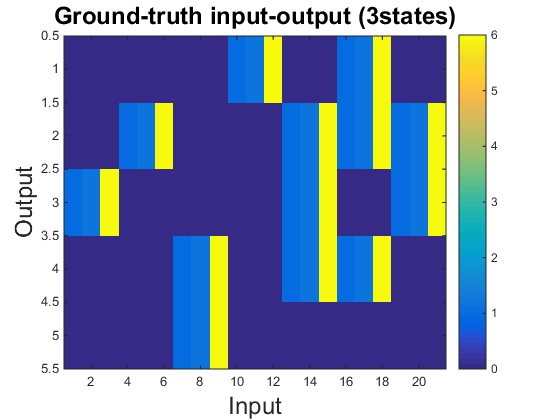
\includegraphics[width=0.3\textwidth]{figure/GT_in_out_3states.png} &   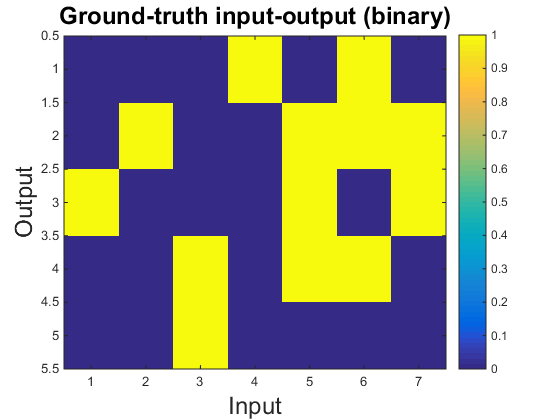
\includegraphics[width=0.3\textwidth]{figure/GT_in_out_bin.png} &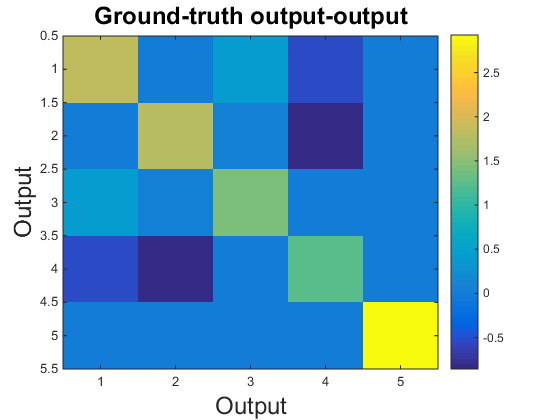
\includegraphics[width=0.3\textwidth]{figure/GT_out_out.png} \\
	(a) & (b)  & (c) \\
		  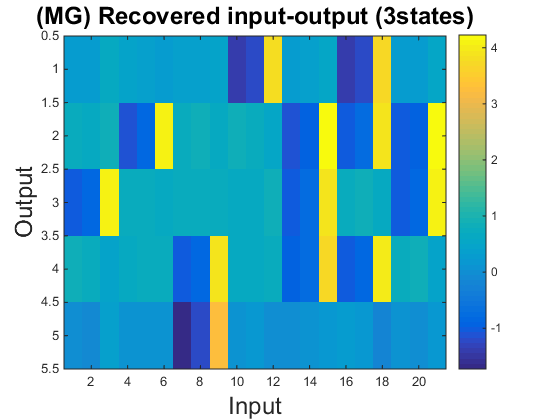
\includegraphics[width=0.3\textwidth]{figure/MGrec_in_out_3states.png} &   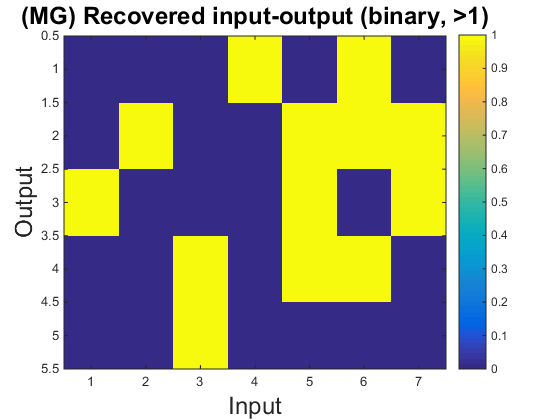
\includegraphics[width=0.3\textwidth]{figure/MGrec_in_out_bin.png} &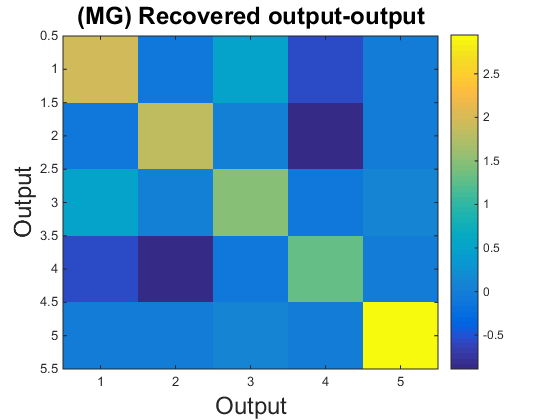
\includegraphics[width=0.3\textwidth]{figure/MG_out_out.png} \\
	(d) & (e) & (f) \\
			  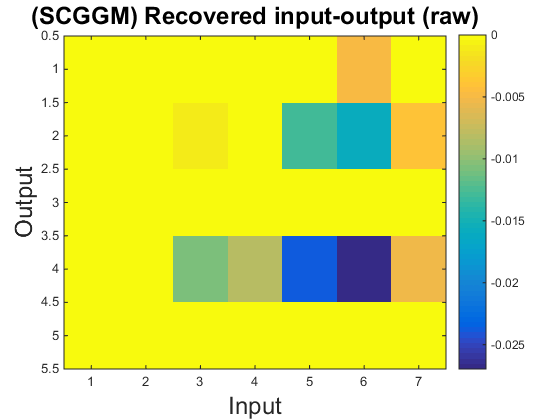
\includegraphics[width=0.3\textwidth]{figure/SCGGMrec_in_out.png} &   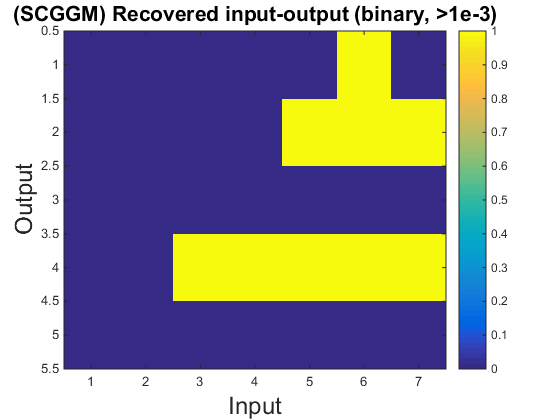
\includegraphics[width=0.3\textwidth]{figure/SCGGMrec_in_out_bin2.png} &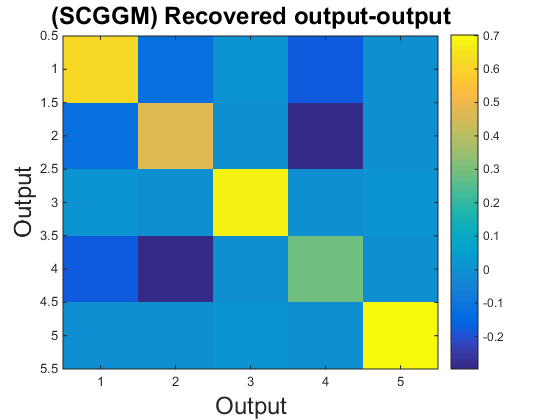
\includegraphics[width=0.3\textwidth]{figure/SCGGM_out_out.png} \\
	(g) & (h)  & (i) \\
	\end{tabular}
	\caption{Ground-Truth (GT) and recovered 'input-output' and 'output-output' interactions of Mixed Graphical model (MG), and sparse CGGM (SCGGM). (a) GT - input-output (3 states), (b) GT - input-output (binary), (c) GT - output-output, (d) MG - input-output (3 states), (e) MG - input-output (binary), (f) MG - output-output, (g) SCGGM - input-output (3 states), (h) SCGGM - input-output (binary), (i) SCGGM - output-output}
	\label{fig:interactions}
\end{figure*}
%\begin{multicols}{2}
%%  \lipsum[3-4]
%\end{multicols}


% % % added for final
% % % end





\subsection{Experiments on Human Liver Cohort Data}
For learning the eQTL mapping between SNPs and the expression rates of the related genes, we use the data from Human Liver Cohort(HLC) study \cite{schadt2008mapping} \footnote{The dataset is downloadable at \url{ https://www.synapse.org/\#!Synapse:syn4499}}. Out of 427 patients with more than 40,000 expression rates and more than 700,000 SNPs in the given data, we first extract 178 samples that contain both information on genotype and expression rates. To focus on learning of the structure of the model rather than handling the huge dimension of this dataset, we focus on smaller subset of genes and expression rates as in the work of Sohn and coworker \cite{sohn2012joint}. We consider only expression rates whose variance is greater than 0.05 and SNPs on chromosome 6 with minor allele frequency greater than 0.01 and pair-wise correlation less than 0.1 to select genes that are not too biased to have major allele and not too related each other according to dbSNP\footnote{\url{http://www.ncbi.nlm.nih.gov/projects/SNP/}}. For a single nucleotide, where major allele is X and minor is Y, SNPs are encoded to categorical variables as XX = 0, XY = 1, YY = 2. SNPs are considered to be discrete variables with three states (0, 1, 2) and expression rates are to be continuous variables in our model. We use 143 samples for training and the remaining 35 samples for testing. For hyperparameter selection, we use 3-fold cross-validation on mean squared error.


\begin{table}
\begin{center}
    \begin{tabular}{| c | c |}
    \hline
    Method & Prediction Error \\
    \hline
    MG & $0.0239$ \\
    SCGGM & $0.0246$  \\
    Lasso & $1.6323 \times 10^{-8}$  \\
    MTLasso & $3.1753 \times 10^{-7}$ \\
    \hline 
    \end{tabular}
\end{center}
\caption{Average prediction error on Human Liver Cohort data testset from Conditional Mixed Graphical Model (MG), Sparse Conditional Gaussian Graphical Model (SCGGM), Lasso, Multi-task Lasso with joint feature selection (MTLasso). The number of SNPs selected is 937 and the number of proteins for expression rates is 100.}
\label{table:real_large}
\end{table}

The prediction error on our model and other baseline models are in Table \ref{table:real_large}. Our method shows lower average prediction error than SCGGM, and this shows that our assumption on genetic variation can be confirmed: the phenotypes of 0 or 1 minor alleles can be drastically different from those with 2 minor alleles, and we need discrete models for SNPs. But the traditional multi-task regression methods (Lasso, MTLasso) shows error much closer to zero. We find the explanation of this discrepancy in error from the sparsity in the parameters in each learned model. The learned coefficient matrix $\textbf{B}$ of Lasso and MTLasso has all non-zero entries, but the input-output mapping learned from MG and SCGGM has very high sparsity. Thus, we see that the Lasso and MTLasso methods make a trade-off for better prediction errors with far less interpretability, and SCGGM and MG converge to a state with very sparse model, only using output-output relationships for better prediction error. We also conjecture that the relatively high sample complexity for our model might be an obstacle for better structure learning. We wanted to further analyze the performance of our method varying settings including hyperparameter candidates and metrics for cross-validation steps, but the learning of our model takes about a week and could not analyze other behaviors on this dataset.

To analyze the behaviors of our model further, we conduct the experiment on selected SNPs and gene expression rates for smaller dimensions. We strengthen the threshold for the selection of SNPs and selected fewer SNPs for our study. We select 36 SNPs with pair-wise correlation is less than 0.01 instead of 0.1. For gene expression rates, we focus on 9 HLA Class II genes following the findings from the previous study \cite{burton2007genome}. The number of samples for training and test and the model selection method are the same as the previous experiment.

\begin{table}
\begin{center}
    \begin{tabular}{| c | c |}
    \hline
    Method & Prediction Error \\
    \hline
    MG & $0.0938$ \\
    SCGGM & $0.0471$  \\
    Lasso & $0.0255$  \\
    MTLasso & $0.0217$ \\
    \hline 
    \end{tabular}
\end{center}
\caption{Average prediction error on selected SNPs and genes from Human Liver Cohort. from Conditional Mixed Graphical Model (MG), Sparse Conditional Gaussian Graphical Model (SCGGM), Lasso, Multi-task Lasso with joint feature selection (MTLasso). The number of SNPs selected is 36 and the number of proteins for expression rates is 9.}
\label{table:real_small}
\end{table}

The prediction error on our model and other baseline models on smaller dataset are in Table \ref{table:real_small}. The prediction errors of SCGGM and our model are worse than that of Lasso, and MTLasso. The sparsity patterns in the coefficient matrix learned from Lasso and MTLasso, and input-output relationship learned from SCGGM and our model are the same as previous experiment. 



\section{Conclusion}
In this project, we adopt conditional mixed graphical model for a better generative model in learning the eQTL mapping in SNPs-gene networks. Our proposed model has two advantages: 1) the relaxation of unnatural assumption in encoding of SNPs in sparse CGGM and 2) the unnecessity of prior knowledge among correlated gene expression rates in each problem settings. Our assumption in the SNPs-gene network is that phenotypes of 0 or 1 minor alleles can be drastically different from those of 2 minor alleles. In synthetic experiments, we confirm that our model outperforms both in prediction error and edge recovery rate when given the data following our assumption. In experiments on Human Liver Cohort dataset, it is hard to decide whether our model performs better than the other baseline models including sparse CGGM and multiple-output regression models, and we conjecture that this is due to relatively high sample complexity of our model. The future work includes developing a faster optimization method than PNOPT and incorporating more refined from of regularization for the discovery of other types of structured sparsity patterns in the network.





\nocite{*}
\bibliographystyle{icml2015}
\bibliography{final}

\end{document}


% This document was modified from the file originally made available by
% Pat Langley and Andrea Danyluk for ICML-2K. This version was
% created by Lise Getoor and Tobias Scheffer, it was slightly modified  
% from the 2010 version by Thorsten Joachims & Johannes Fuernkranz, 
% slightly modified from the 2009 version by Kiri Wagstaff and 
% Sam Roweis's 2008 version, which is slightly modified from 
% Prasad Tadepalli's 2007 version which is a lightly 
% changed version of the previous year's version by Andrew Moore, 
% which was in turn edited from those of Kristian Kersting and 
% Codrina Lauth. Alex Smola contributed to the algorithmic style files.  
